\documentclass[12pt]{article}

\usepackage{amsmath}
\usepackage{listings}
\usepackage{tikz}

\lstset{frame=tb,
  language=octave,
  basicstyle={\small\ttfamily},
  tabsize=2
}

\title{EECS 477 HW1}
\author{Andrew Mason}

\begin{document}
\maketitle
\begin{enumerate}
  \item
    \begin{enumerate}
      \item
        \begin{enumerate}
          \item
            On an $n$ vertex star graph, the algorithm will first select the
            vertex in the center of the star, since it has degree $n-1$, while
            all other vertices in the graph have degree $1$. After removing all
            edges incident on the central vertex, the graph has no remaining
            edges, and the vertex cover contains just one vertex. This is
            optimal for this graph, since the vertex cover cannot be empty if
            the graph has at least one edge, so a vertex cover of size $1$ is
            the smallest possible vertex cover.
          \item
            On a $K_4$ minus one edge, there are two vertices of degree $3$,
            and two vertices of degree $2$. The algorithm will pick one of the
            degree-$3$ vertices. Since this vertex has an edge to every other
            vertex in the graph (its degree is $|V| - 1$), removing its
            incident edges will reduce the degree of every other vertex by $1$.
            Now, there is one vertex with degree $2$, and two with degree $1$.
            The algorithm will select the degree-$2$ vertex, and, upon removing
            its incident edges, the vertex cover will be complete with size
            $2$. This is optimal, because a vertex cover of size $1$ is not
            possible. If we select just one of the degree-$2$ vertices, we miss
            at least the edge connecting the two degree-$3$ vertices. If we
            select one of the degree-$3$ vertices, we know that we are missing
            some edges, because this is the choice that our algorithm made, but
            the algorithm did not stop here because there were still edges in
            the graph.
        \end{enumerate}
      \item
        The following figure illustrates a graph that demonstrates that the
        described algorithm is worse than a 2-approximation algorithm. First,
        the edges should be undirected (I used an online tool - http://madebyevan.com/fsm/
        - and it only draws arrows).\\
        This graph has an optimal vertex cover of 6 (the set of six vertices in
        the second column from the left), but in the worst case, depending on
        how a few ties are broken when choosing between two vertices with equal
        degree, the algorithm gives a vertex cover of size 13 (consisting of
        every vertex except those belonging to the optimal vertex cover).
        \begin{center}
        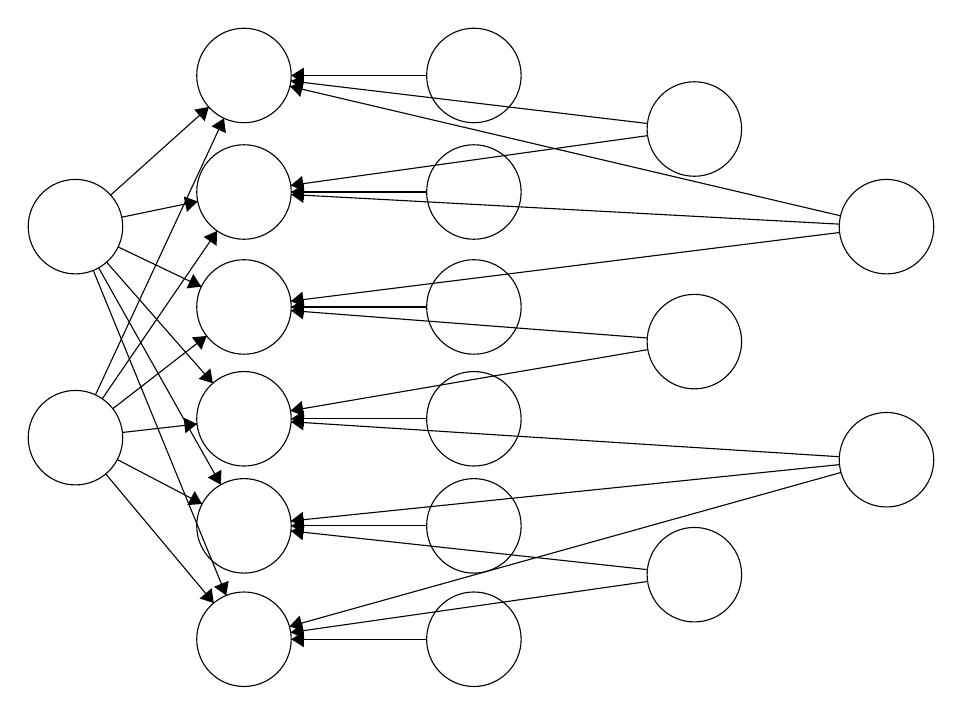
\begin{tikzpicture}[scale=0.2]
        \tikzstyle{every node}+=[inner sep=0pt]
        \draw [black] (55.5,-23.4) circle (3);
        \draw [black] (14.7,-13.8) circle (3);
        \draw [black] (14.7,-21.2) circle (3);
        \draw [black] (14.7,-28.5) circle (3);
        \draw [black] (14.7,-35.6) circle (3);
        \draw [black] (14.7,-42.4) circle (3);
        \draw [black] (14.7,-49.6) circle (3);
        \draw [black] (29.3,-13.8) circle (3);
        \draw [black] (29.3,-21.2) circle (3);
        \draw [black] (29.3,-28.5) circle (3);
        \draw [black] (29.3,-35.6) circle (3);
        \draw [black] (29.3,-42.4) circle (3);
        \draw [black] (29.3,-49.6) circle (3);
        \draw [black] (43.3,-17.2) circle (3);
        \draw [black] (43.3,-30.7) circle (3);
        \draw [black] (43.3,-45.5) circle (3);
        \draw [black] (55.5,-38.2) circle (3);
        \draw [black] (4,-23.4) circle (3);
        \draw [black] (4,-36.8) circle (3);
        \draw [black] (40.33,-45.93) -- (17.67,-49.17);
        \fill [black] (17.67,-49.17) -- (18.53,-49.56) -- (18.39,-48.57);
        \draw [black] (40.32,-45.18) -- (17.68,-42.72);
        \fill [black] (17.68,-42.72) -- (18.42,-43.31) -- (18.53,-42.31);
        \draw [black] (40.34,-31.21) -- (17.66,-35.09);
        \fill [black] (17.66,-35.09) -- (18.53,-35.45) -- (18.36,-34.47);
        \draw [black] (40.31,-30.47) -- (17.69,-28.73);
        \fill [black] (17.69,-28.73) -- (18.45,-29.29) -- (18.53,-28.29);
        \draw [black] (26.3,-49.6) -- (17.7,-49.6);
        \fill [black] (17.7,-49.6) -- (18.5,-50.1) -- (18.5,-49.1);
        \draw [black] (26.3,-42.4) -- (17.7,-42.4);
        \fill [black] (17.7,-42.4) -- (18.5,-42.9) -- (18.5,-41.9);
        \draw [black] (26.3,-35.6) -- (17.7,-35.6);
        \fill [black] (17.7,-35.6) -- (18.5,-36.1) -- (18.5,-35.1);
        \draw [black] (26.3,-28.5) -- (17.7,-28.5);
        \fill [black] (17.7,-28.5) -- (18.5,-29) -- (18.5,-28);
        \draw [black] (26.3,-21.2) -- (17.7,-21.2);
        \fill [black] (17.7,-21.2) -- (18.5,-21.7) -- (18.5,-20.7);
        \draw [black] (26.3,-13.8) -- (17.7,-13.8);
        \fill [black] (17.7,-13.8) -- (18.5,-14.3) -- (18.5,-13.3);
        \draw [black] (40.33,-17.62) -- (17.67,-20.78);
        \fill [black] (17.67,-20.78) -- (18.53,-21.17) -- (18.39,-20.18);
        \draw [black] (40.32,-16.85) -- (17.68,-14.15);
        \fill [black] (17.68,-14.15) -- (18.41,-14.75) -- (18.53,-13.75);
        \draw [black] (52.58,-22.71) -- (17.62,-14.49);
        \fill [black] (17.62,-14.49) -- (18.28,-15.16) -- (18.51,-14.18);
        \draw [black] (52.5,-23.24) -- (17.7,-21.36);
        \fill [black] (17.7,-21.36) -- (18.47,-21.9) -- (18.52,-20.91);
        \draw [black] (52.52,-23.77) -- (17.68,-28.13);
        \fill [black] (17.68,-28.13) -- (18.53,-28.52) -- (18.41,-27.53);
        \draw [black] (52.51,-38.01) -- (17.69,-35.79);
        \fill [black] (17.69,-35.79) -- (18.46,-36.34) -- (18.52,-35.34);
        \draw [black] (52.52,-38.51) -- (17.68,-42.09);
        \fill [black] (17.68,-42.09) -- (18.53,-42.51) -- (18.43,-41.51);
        \draw [black] (52.61,-39.01) -- (17.59,-48.79);
        \fill [black] (17.59,-48.79) -- (18.49,-49.06) -- (18.23,-48.1);
        \draw [black] (6.23,-21.4) -- (12.47,-15.8);
        \fill [black] (12.47,-15.8) -- (11.54,-15.97) -- (12.21,-16.71);
        \draw [black] (6.94,-22.8) -- (11.76,-21.8);
        \fill [black] (11.76,-21.8) -- (10.88,-21.48) -- (11.08,-22.46);
        \draw [black] (6.71,-24.69) -- (11.99,-27.21);
        \fill [black] (11.99,-27.21) -- (11.48,-26.41) -- (11.05,-27.32);
        \draw [black] (5.98,-25.66) -- (12.72,-33.34);
        \fill [black] (12.72,-33.34) -- (12.57,-32.41) -- (11.82,-33.07);
        \draw [black] (5.47,-26.01) -- (13.23,-39.79);
        \fill [black] (13.23,-39.79) -- (13.27,-38.84) -- (12.4,-39.33);
        \draw [black] (5.13,-26.18) -- (13.57,-46.82);
        \fill [black] (13.57,-46.82) -- (13.73,-45.89) -- (12.8,-46.27);
        \draw [black] (5.92,-39.1) -- (12.78,-47.3);
        \fill [black] (12.78,-47.3) -- (12.65,-46.36) -- (11.88,-47.01);
        \draw [black] (6.66,-38.19) -- (12.04,-41.01);
        \fill [black] (12.04,-41.01) -- (11.57,-40.19) -- (11.1,-41.08);
        \draw [black] (6.98,-36.47) -- (11.72,-35.93);
        \fill [black] (11.72,-35.93) -- (10.87,-35.53) -- (10.98,-36.52);
        \draw [black] (6.37,-34.96) -- (12.33,-30.34);
        \fill [black] (12.33,-30.34) -- (11.39,-30.43) -- (12,-31.22);
        \draw [black] (5.7,-34.33) -- (13,-23.67);
        \fill [black] (13,-23.67) -- (12.14,-24.05) -- (12.96,-24.62);
        \draw [black] (5.27,-34.08) -- (13.43,-16.52);
        \fill [black] (13.43,-16.52) -- (12.64,-17.03) -- (13.55,-17.46);
        \end{tikzpicture}
        \end{center}
    \end{enumerate}
  \item
    \begin{enumerate}
      \item
        \begin{equation}
          \begin{split}
            \text{min }& -3x_1 + 5x_2 \\
            \text{s.t. }& 4x_1 + 5x_2 - s = 3 \\
            & 6x_1 - 6x_2 = 7 \\
            & x_1 + 8x_2 + t = 20 \\
            & x_1, x_2, s, t\geq 0 \\
          \end{split}
        \end{equation}
      \item
        \begin{lstlisting}
        # problem2.m
        c = [3, -5]';
        A = [4, 5;
             6, -6;
             1, 8];
        b = [3, 7, 20]';
        lb = [0, 0];
        ub = [];
        ctype = "LSU";
        vartype = "CC";
        sense = -1;
        [xmax, fmax, status, extra] = ...
          glpk(c, A, b, lb, ub, ctype, vartype, sense);
        disp(xmax);
        \end{lstlisting}

        The solution to the original LP is $(x_1, x_2) = (1.16667, 0.00000)$.\\
    \end{enumerate}
  \item
    The integer linear program can be solved with the following octave code.\\
    \begin{lstlisting}
      # problem3.m
      c = [3, -5]';
      A = [4, 5;
           6, -6;
           1, 8];
      b = [3, 7, 20]';
      lb = [0, 0];
      ub = [];
      ctype = "LSU";
      vartype = "II";
      sense = -1;
      [xmax, fmax, status, extra] = ...
        glpk(c, A, b, lb, ub, ctype, vartype, sense);
      disp(xmax);
    \end{lstlisting}

    The solution is $(x_1, x_2) = (0, 0)$.\\
  \item
    The knapsack problem can be formulated as the following linear program.\\
    \begin{equation}
      \begin{split}
      \text{max } & 30x_1 + 20x_2 + 100x_3 + 90x_4 + 160x_5 \\
      \text{s.t. } & 5x_1 + 10x_2 + 20x_3 + 30x_4 + 50x_5\leq 60 \\
      & 0\leq x_1, x_2, x_3, x_4, x_5\leq 1 \\
      \end{split}
    \end{equation}
    And can be solved with the following octave code.\\
    \begin{lstlisting}
      # problem4.m
      c = [30, 20, 100, 90, 160]';
      A = [5, 10, 20, 30, 40];
      b = [60]';
      lb = [0, 0, 0, 0, 0];
      ub = [1, 1, 1, 1, 1];
      ctype = "U";
      vartype = "CCCCC";
      sense = -1;

      [xmax, fmax, status, extra] = ...
        glpk(c, A, b, lb, ub, ctype, vartype, sense);
      disp(xmax);
    \end{lstlisting}
    Which gives the solution $x_1 = 1; x_3 = 1;x_5 = 0.875;x_2,x_4 = 0$.\\
  \item
    The knapsack problem can be formulated as the following integer linear program.\\
    \begin{equation}
      \begin{split}
      \text{max } & 30x_1 + 20x_2 + 100x_3 + 90x_4 + 160x_5 \\
      \text{s.t. } & 5x_1 + 10x_2 + 20x_3 + 30x_4 + 50x_5\leq 60 \\
      & 0\leq x_1, x_2, x_3, x_4, x_5\leq 1 \\
      & x_1, x_2, x_3, x_4, x_5 \text{ integer} \\
      \end{split}
    \end{equation}
    And can be solved with the following octave code.\\
    \begin{lstlisting}
      # problem5.m
      c = [30, 20, 100, 90, 160]';
      A = [5, 10, 20, 30, 40];
      b = [60]';
      lb = [0, 0, 0, 0, 0];
      ub = [1, 1, 1, 1, 1];
      ctype = "U";
      vartype = "IIIII";
      sense = -1;

      [xmax, fmax, status, extra] = ...
        glpk(c, A, b, lb, ub, ctype, vartype, sense);
      disp(xmax);
    \end{lstlisting}
    Which gives the solution $x_3 = 1;x_5 = 1;x_1,x_2,x_4 = 0$.\\

    In the fractional version, one way to reach the optimal is to fill the
    knapsack with as much as possible of $x_i$, going in decreasing order of
    the profit-to-weight ratios of each $x_i$. In the integer version, this
    cannot be used as the strategy, because there is the possibility that the
    last item added to the knapsack will not completely fit, which would result
    in lost value from the unused capacity. So, the integer solution appears to
    choose higher absolute value that exactly fill the knapsack ($x_3$ and $x_5$,
    in this case) over higher values normalized by weight.
  \item
    $F/I$ can be made arbitrarily large when $I > 0$. Consider the following
    knapsack problem:\\
    \begin{equation}
      \begin{split}
      \text{max }& x_1 + kx_2 \\
      \text{s.t. }& x_1 + wx_2\leq w - 1 \\
      & 0\leq x_1,x_2\leq 1 \\
      & 1 < w < k \\
      \end{split}
    \end{equation}
    In the integer version, $x_2$ cannot be included in the knapsack by
    construction. But in the fractional version, $\frac{w-1}{w}$ of $x_2$ will
    fill the knapsack. In this way, the ratio $F/I$ is defined as $k\frac{w-1}{w}$.
    So by letting $k$ grow larger, $F/I$ can be made arbitrarily large. You can
    view the code in ``problem6.m'' for one example of this.
  \item
    \begin{enumerate}
      \item
        One way to formulate this problem is to say that the decision variable
        $x_{ij}$ is the number of teams hired from contractor $i$ in region $j$.
        Additionally, assume that an additional input to the program - $k$ -
        specificies that $\forall i<k c_i$ is experienced, while all other
        contractors are not. This yields the following generalization of the problem.\\
        \begin{equation}
          \begin{split}
            \text{min } &\sum_{i}\sum_{j} c_{ij}x_{ij} \\
            \text{s.t. } &\forall i \sum_{j} x_{ij}\leq u_i \\
            & \forall j\sum_{i}^{k}x_{ij}\geq 1 \\
            & \forall j\sum_{i}x_{ij}\geq r_j \\
            & \forall i,j\text{ }x_{ij}\geq 0 \\
            & \forall i,j\text{ }x_{ij}\text{ integer} \\
          \end{split}
        \end{equation}
      \item
        The linear relaxation therefore is:\\
        \begin{equation}
          \begin{split}
            \text{min } &\sum_{i}\sum_{j} c_{ij}x_{ij} \\
            \text{s.t. } &\forall i \sum_{j} x_{ij}\leq u_i \\
            & \forall j\sum_{i}^{k}x_{ij}\geq 1 \\
            & \forall j\sum_{i}x_{ij}\geq r_j \\
            & \forall i,j\text{ }x_{ij}\geq 0 \\
          \end{split}
        \end{equation}
      \item
        See the included octave file (problem7.m) for the 5 documented attempts.
        In my attempts, I was attempting to make the cheaper contractors more
        scarce, hoping that the regions would divy up fractions of the cheaper
        contractors amongst themselves before moving on to the more expensive
        contractors. Unfortunately, this did not yield a successful result, even
        when the cheaper contractors were made the more experienced ones.
    \end{enumerate}
\end{enumerate}
\end{document}
